Text-aware process prediction aims to utilize unstructured text information in event data to improve predictions for unfinished cases.
While many prediction methods have been applied to event data, almost none of them are able to handle textual data.
An exception is the approach presented in \cite{DBLP:conf/bpm/TeinemaaDMF16}, where traces with text data are encoded as fixed vectors and a classifier is learned for each prefix length.

In this chapter a novel approach for process prediction is presented that considers control flow, additional numerical, categorical and textual data, captures temporal dependencies, seasonal variability and concept drifts using an event-wise encoding and a sequential prediction model (LSTM).

\section{Overview}

The proposed framework consists of a preprocessing, encoding and prediction model component, which operate in an offline and online phase.
The encoding component distinguish between categorical or numerical data that can be encoded directly and textual data, which requires a textual model.

In the offline phase a historical event log with completed traces of a business process is used to train the prediction model.
Given an event log $\eventlog = \{\sigma_1, \dots, \sigma_l\}$ with historical event data, the set of all prefix traces $\eventlog_\mathrm{prefix} = \{\sigma(1,k) \mid \forall \sigma \in \eventlog, 1 \leq k \leq |\sigma|\}$ is computed.
Each prefix with the desired target value corresponds to one training example for the prediction model.
The total number of training examples that can be generated out of the log is $\sum_{\sigma \in \eventlog}|\sigma|$, which is exactly the number of events in the log.

As target the activity and timestamp (relative to case start) of the next event as well as the outcome and cycle time (time between first and last event) of the case is chosen.
For completed cases the next event's activity is an artificial "<Process End>" with the same timestamp as the final event.

The text data of the historical log is extracted to build a text corpus and construct a text model.

The prefix traces are encoded to sequences of fixed-length event vectors using the text model.




\begin{figure}
	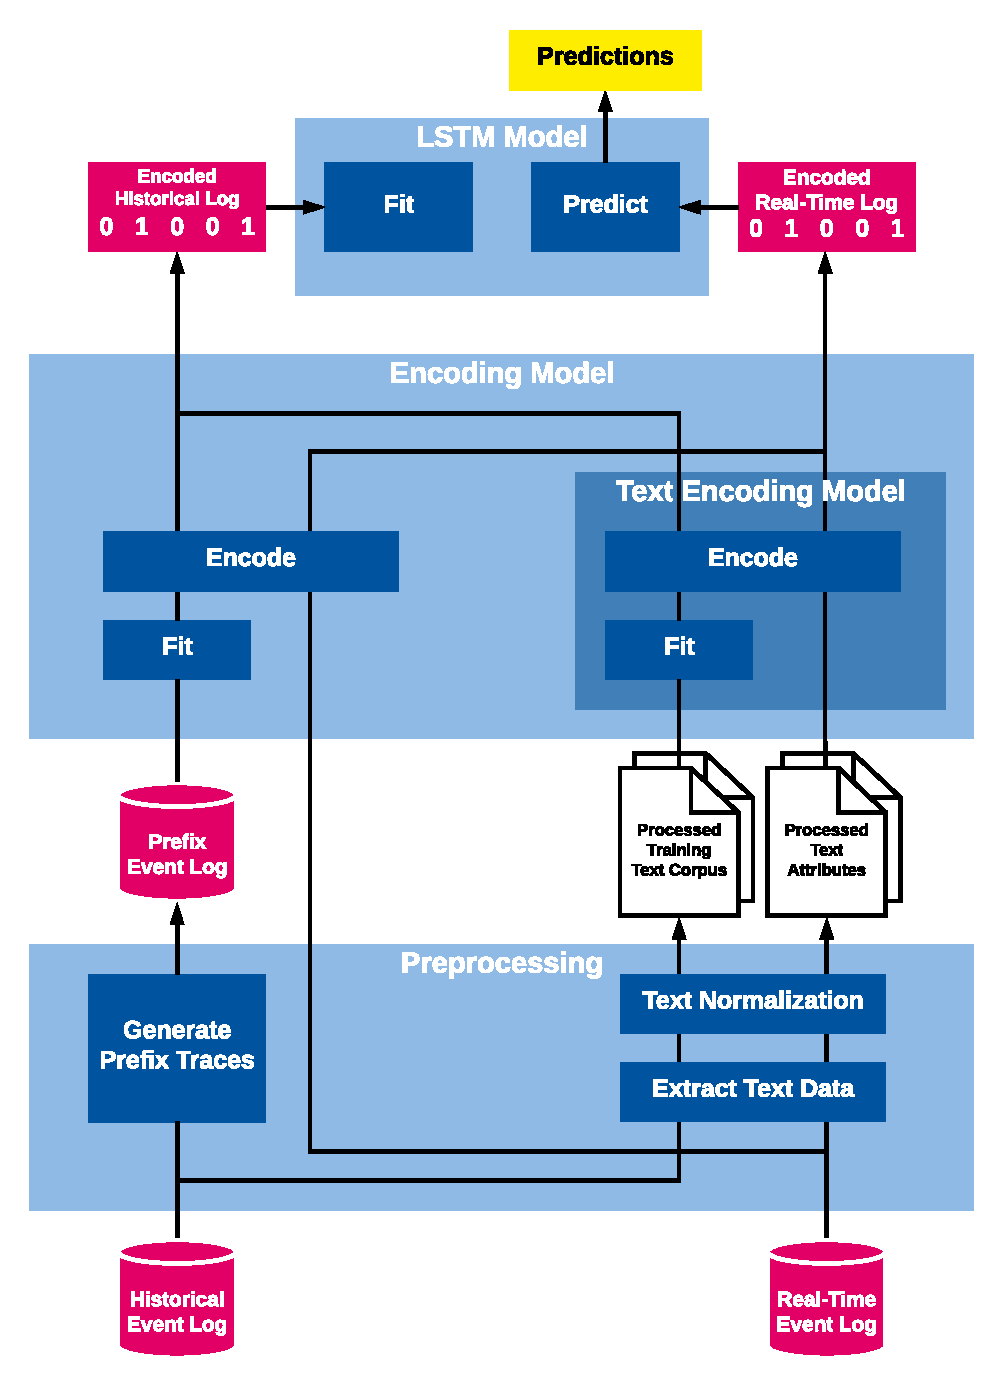
\includegraphics[width=\textwidth]{figures/framework}
	\caption{Framework}
	\label{fig:framework}
\end{figure}


\section{Event Encoding}

In the offline training phase as well as during online prediction, traces are encoded as sequences of event vectors.
Each event is encoded as a fixed-length vector using the event's activity, timestamp and additional categorical, numerical and textual attributes.
The encoded event vector is the concatenation of feature vectors, which are constructed from the event data.

The activity of an event is represented using \textit{one-hot encoding}.
Given the set of possible activities $\mathcal{A}$, an arbitrary but fixed ordering over is introduced with a bijective index function $index_\mathcal{A} \in \mathcal{A} \rightarrow \{1, \dots, |\mathcal{A}|\}$.
Using this function, the activity is encoded as a vector of size $|\mathcal{A}|$, where the component $index_\mathcal{A}(\pi_\mathcal{A}(e))$ has value 1 and all the other components have value 0.
We write $\mathds{1}$

The timestamp of an event is used to compute a set of time-related features, which is 




\begin{equation}
	\bm{x_e}=(
	\bm{a}_e,
	\bm{t}_e,
	\bm{d}_1^\mathrm{num}, \dots,\bm{d}_r^\mathrm{num},
	\bm{d}_1^\mathrm{cat}, \dots,\bm{d}_s^\mathrm{cat},
	\bm{d}_1^\mathrm{text}, \dots, \bm{d}_u^\mathrm{text})
\end{equation}


\begin{table}[!htbp]

\begin{tabularx}{\textwidth}{p{2cm} l l p{10cm} }
	\toprule
	 \textbf{Feature} \newline \textbf{Vector} & \textbf{Construction} &\textbf{Dimension} &  \textbf{Description} \\
	 \midrule
	 	$\bm{a}$ &$\mathds{1}(\pi_\mathcal{A}(e))$& $|\mathcal{A}|$& One-hot encoding of the activity. \\
	 	$\bm{t}$ & See Section \ref{sec:time} &6 & Time-based feature vector.\\
	 	$\bm{d}_i^\mathrm{num}$ & &1 & Normalized value of the $i$-th numerical attribute\\
	 	$\bm{d}_i^\mathrm{cat}$ & $\mathds{1}(\pi_{{\mathcal{D}_i}^\mathrm{cat}}(e))$&$|\mathcal{D}_i|$ & One-hot encoding of the $i$-th categorical attribute.\\
	 	$\bm{d}_i^\mathrm{text}$ & See Section \ref{sec:text} & $z_i$& Fixed-length vectorization of the $i$-th text attribute.\\
	\bottomrule
\end{tabularx}
	\caption{Feature vectors for event encoding.}
	\label{tab:features}
\end{table}

\begin{equation}
	|\bm{x}_e|= |\mathcal{A}| + r + \sum_{i=1}^{s} |\mathcal{D}_i| + \sum_{j=1}^{u} z_j + 6
\end{equation}


\section{Capturing Temporal Dependencies}\label{sec:time}


For timestamp prediction of the next and final event of running process instance a set of time-based features is computed from the timestamp data in the event log.
Given an event log $\eventlog$ an event $e_i$ from a trace $\sigma = \langle e_1, \dots, e_n \rangle$ the following time features are computed for the encoding of $e_i$: 

\begin{center}
\begin{tabularx}{\textwidth}{l l}
	\centering
	 \textbf{Feature} & \textbf{Description} \\
	$t_1 = \pi_\mathcal{T}(e_i) - \pi_\mathcal{T}(e_{i-1})$ & Seconds since previous event \\
	$t_2 = \pi_\mathcal{T}(e_i) - \pi_\mathcal{T}(e_1)$ & Seconds since case start \\
	$t_3 = \pi_\mathcal{T}(e_i) - \min\{\pi_\mathcal{T}(e_{j}), \forall e_j \in \sigma_k, \forall  \sigma_k \in \eventlog\}$ & Seconds since first recorded event \\
	$t_4$ & Seconds since midnight \\
	$t_5$ & Seconds since last Monday \\
	$t_6$ & Seconds since last January 1 00:00
\end{tabularx}
\end{center}

Using the time features a set of time-dependent trends can be captured and utilized for prediction.
The features $t_1$ and $t_2$ give information about the time between events and the time of the event in the case.
Using $t_3$ the absolute time position of an event in the data can be determined.
This is important to detect concept drift in the process.
The features $t_4, t_5$ and $t_6$ are used to capture daily, weekly or seasonal trends.
For example, some activities might only be executed during office hours, before the weekend, during summer.

Each feature $t_1, \dots t_6$ as well as all additional numerical attributes $d_i$ are scaled to the interval $ [0, 1]$ to improve learning efficiency using min-max normalizing.
The scaling for a numerical feature $x$ is realized with the transformation

$$\hat{x} = \dfrac{x-\min(x)}{\max(x) - \min(x)},$$

where $\min(x)$ is the lowest and $\max(x)$ is the highest value $x$ can take.
If the limits are not bounded conceptually, the lowest or highest value of $x$ in the event log is used for scaling.

\section{Text Vectorization}\label{sec:text}

In order to prepare the textual data of the event log for a prediction model, the texts have to be encoded in a compact, finite and "useful" numerical vector representationu using a text model.
Useful in that context means, that texts with similar semantic meanings should also have similar representations.
The vector representation of text data is an important aspect in \textit{Natural Language Processing} (NLP).
Extracting the meaning of textual information remains a challenge even for humans, because textual data is unstructured, language dependent and domain specific.
Many words are ambiguous, for example the word "apple" might denote a fruit or a global technology company.
In addition, grammatical variations and the importance of context in language makes extracting the semantic meaning even more difficult for computers.


In our setting, the text vectorization is realized in a 2-step procedure.
First, all text data associated with the events in the corresponding textual attribute is collected in a so called \textit{text corpus}.
Each document in the text corpus is then preprocessed in order to filter out linguistic noise or useless information.
Finally, the text corpus is used to build up a vocabulary and a text vectorization technique is applied to encode the text attribute to a fixed of vector.

\subsection{Text Preprocessing}

In the preprocessing step each document is transformed by a processing pipeline which consists of the following four steps:

\begin{enumerate} 
	\item Letters are converted to lowercase
	\item Document is tokenized by word
	\item Each word is lemmatized
	\item Stop words are filtered out
\end{enumerate}

In the tokenenization step a document is split up in a list of words.
Each word is then lemmatized, i.e. it is converted to its canonical form.
The idea is to unify words that have a very similar meaning and filter out grammatical variations.
For example, the words  "go", "going", "goes", "gone" and "went" are all transformed to the basic form "go".
Ultimately, all stop words are filtered out of each document.
Stop words are words with low information value like "the", "a", "of" or "here".

Stop word lists are language dependent and can be more or less aggressive at filtering.
Usually they contains articles, auxiliary verbs, prepositions and generic verbs like "be" and "have".
In addition, punctuation marks or numerical information are excluded.

\begin{table}[]
	\begin{tabularx}{\textwidth}{l l p{9.8cm}}
		\toprule
		\textbf{Step} & \textbf{Transformation} & \textbf{Document}                                                       \\ \midrule
		0             & Original       & "The patient has been diagnosed with high blood pressure." \\
		1             & Lowercase               & "the patient has been diagnosed with high blood pressure." \\
		2 & Tokenization  & {[}"the", "patient", "has", "been", "diagnosed", "with", "high", "blood", "pressure", "."{]} \\
		3 & Lemmatization & {[}"the", "patient", "have", "be", "diagnose", "with", "high", "blood", "pressure", "."{]}   \\
		4             & Stop word filtering     & {[}"patient", "diagnose", "high", "blood", "pressure"{]} \\ \bottomrule
	\end{tabularx}
	\caption{Preprocessing transformation of an example document.}
	\label{tab:text-preprocessing}
\end{table}







\subsection{Bag-of-Words}

The \textit{bag-of-words} (BoW) Model is a simple text model, which represents documents based on the \textit{term frequencies} of its words.
Given the learned vocabulary $V$ a document is represented by a vector of size $|V|$, where the $i$-th component gives the number of occurrences of the word indexed with $i$ in the document.

Since this approach does not reflect the prior distributions of words in the corpus, i.e. how likely certain words appear in a document, the term frequencies are usually normalized by the so-called \textit{inverse document frequency} of a word.
The inverse document frequency indicates the specificity of a word in the corpus and is computed by dividing the total number of documents by the number of documents that contain the specific word and scaling that value logarithmically.

The bag-of-words model is easy to build and effective for certain applications, but limited in several ways.
First, the model completely ignores the order of words, which is often crucial for understanding the semantic meaning. For example, the sentences "The patient's health state went from stable to critical." and "The patient's health state went from critical to stable." would result in the same vector representation, while the meaning is clearly inverted.
Second, the vector representations are sparse and of high dimensionality since they depend of the size of the vocabulary.
However, the dimension can be reduced by limiting the size of the vocabulary. For example, this can be realized for exampand omit certain words.

\subsection{Bag-of-N-Grams}

The \textit{bag-of-n-grams} model is a generalization of the Bag-of-Words model, which addresses the missing word order awareness of the latter.
Instead of single words, the vocabulary consists of $n$-tuples of words, that appear consecutive in the corpus.
The unigram model ($n=1$) is equivalent to the BoW model.


\subsection{Paragraph Vector}
\subsection{Latent Dirichlet Allocation}

\section{Network Architecture and Training}

\section{Online Prediction}